\section{Measurement and Results}
As mentioned above, this experiment has 3 different sets of measurements: 
\begin{itemize}
    \item \textbf{Measurement of Correlation Functions}
    \item \textbf{Violation of Bell’s Inequality}
    \item \textbf{Quantum State Tomography}
\end{itemize}

Thus, this section is also divided into 3 different sections. Each subsection is dedicated to one of the following.

\subsection{Correlation Functions}
In the first part of the experiment, the aim is to measure correlation functions for 2 different cases. In both cases, there are 2 different half-wave plates. One half-wave plate ($HWP_{B}$) is located in the pathway of the photon that goes to Bob, and the other one ($HWP_{A}$) is located in the pathway of the photon that goes to Alice. The angles of the half-wave plates are as follows: 
\begin{itemize}
    \item {Case 1}:
        $\alpha_{HWP_{B}}$ = 0$^\circ$, $\alpha_{HWP_{A}}$ = $i^\circ$ ($i \in$ \{0, 10, 20, 30, 40, 50, 60, 70, 80, 90\})
    \item {Case 2}:
        $\alpha_{HWP_{B}}$ = 22.5$^\circ$, $\alpha_{HWP_{A}}$ = $i^\circ$ ($i \in$ \{0, 10, 20, 30, 40, 50, 60, 70, 80, 90\})
\end{itemize}
For both cases, the angles for the half-wave plates were changed by rotating the half-wave plate. After each configuration, coincidence counts were recorded by the help of a C++ script. Counts for each state and case can be seen below:

% Table for the coincidence counts for the first case
\begin{table}[h!]
    \centering
    \begin{tabular}{|c|c|c|c|c|c|c|c|c|c|c|}
        \hline
        $\alpha_{HWP_{A}}$ & 0$^\circ$ & 10$^\circ$ & 20$^\circ$ & 30$^\circ$ & 40$^\circ$ & 50$^\circ$ & 60$^\circ$ & 70$^\circ$ & 80$^\circ$ & 90$^\circ$ \\
        \hline
        $C_{HH}$ & 251 & 197 & 164 & 76 & 29 & 9 & 28 & 113 & 187 & 216 \\
        $C_{HV}$ & 6 & 18 & 67 & 133 & 196 & 195 & 173 & 111 & 45 & 8 \\
        $C_{VH}$ & 5 & 8 & 67 & 135 & 206 & 232 & 225 & 127 & 56 & 7 \\
        $C_{VV}$ & 205 & 199 & 165 & 73 & 22 & 10 & 36 & 88 & 162 & 234 \\
        \hline
    \end{tabular}
    \caption{Coincidence counts for the first case where $\alpha_{HWP_{B}}$ = 0$^\circ$.}
    \label{tab:coincidence_counts_case1}
\end{table}

\begin{table}[h!]
    \centering
    \begin{tabular}{|c|c|c|c|c|c|c|c|c|c|c|}
        \hline
        $\alpha_{HWP_{A}}$ & 0$^\circ$ & 10$^\circ$ & 20$^\circ$ & 30$^\circ$ & 40$^\circ$ & 50$^\circ$ & 60$^\circ$ & 70$^\circ$ & 80$^\circ$ & 90$^\circ$ \\
        \hline
        $C_{HH}$ & 101 & 161 & 167 & 139 & 108 & 42 & 14 & 25 & 48 & 111 \\
        $C_{HV}$ & 105 & 50 & 26 & 30 & 76 & 154 & 190 & 199 & 155 & 112 \\
        $C_{VH}$ & 86 & 45 & 18 & 42 & 91 & 167 & 186 & 180 & 126 & 82 \\
        $C_{VV}$ & 106 & 183 & 222 & 199 & 157 & 98 & 37 & 21 & 62 & 135 \\
        \hline
    \end{tabular}
    \caption{Coincidence counts for the second case where $\alpha_{HWP_{B}}$ = 22.5$^\circ$.}
    \label{tab:coincidence_counts_case2}
\end{table}

\subsubsection{Calculation of Correlation Functions}
To calculate the correlation values, first we need to calculate relative frequencies for each state. Relative frequencies are calculated by dividing the coincidence counts by the total number of counts:
\begin{equation}
    f_{ij} = \frac{C_{ij}}{\sum_{i,j} C_{ij}} \quad (i,j \in \{H, V\})
\end{equation}

After calculating the relative frequencies, we can calculate the correlation values using the following formula with the relative frequencies from \hyperref[tab:coincidence_counts_case1]{Table \ref*{tab:coincidence_counts_case1}} and \hyperref[tab:coincidence_counts_case2]{Table \ref*{tab:coincidence_counts_case2}}:
\begin{equation}
    K_{ij}^{ex} = f_{HH} - f_{HV} - f_{VH} + f_{VV}
\end{equation}
with $i, j \in \{H, V\}$. Correlation values for both cases can be seen below:
\begin{table}[h!]
    \centering
    \begin{tabular}{|c|c|c|c|c|c|c|c|c|c|c|}
        \hline
        $\alpha_{HWP_{A}}$ & 0$^\circ$ & 10$^\circ$ & 20$^\circ$ & 30$^\circ$ & 40$^\circ$ & 50$^\circ$ & 60$^\circ$ & 70$^\circ$ & 80$^\circ$ & 90$^\circ$ \\
        \hline
        $Case~1$ & 0.953 & 0.877 & 0.421 & -0.279 & -0.775 & -0.915 & -0.723 & -0.084 & 0.551 & 0.936 \\ 
        $Case~2$ & 0.040 & 0.567 & 0.797 & 0.648  & 0.227  & -0.393 & -0.761 & -0.784 & -0.437 & 0.118 \\
        \hline
    \end{tabular}
    \caption{Calculated correlation values.}
    \label{tab:correlation_values}
\end{table}

\subsubsection{Visibility}
The visibility can be used to parameterize the contrast of measured graphs \cite{manual}. It is defined as the ratio of the difference between the maximum and minimum value of the correlation function to the sum of the maximum and minimum values.
Since a correlation function can be bounded by -1 and 1, the visibility of this function would lead to $\frac{2}{0}$ in a perfect experimental setup. This is why we need to fit the correlation function to a function to calculate the visibility. Since the correlation function is a sinusoidal function, we can fit it to a sinusoidal function. The fit function is given as:
\begin{equation}
    f(\theta) = A \cdot \sin(B \cdot \theta + C) + D
\end{equation}
The fits for both cases can be seen below:
\begin{figure}[h!]
    \centering
    \begin{subfigure}[t]{0.45\textwidth}
        \centering
        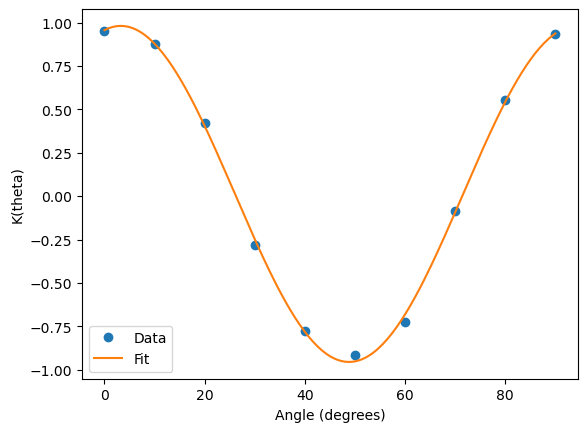
\includegraphics[width=\textwidth]{figures/fit_1.png}
        \caption{Fit for the first case.}
        \label{fig:fit_1}
    \end{subfigure}
    \hfill
    \begin{subfigure}[t]{0.45\textwidth}
        \centering
        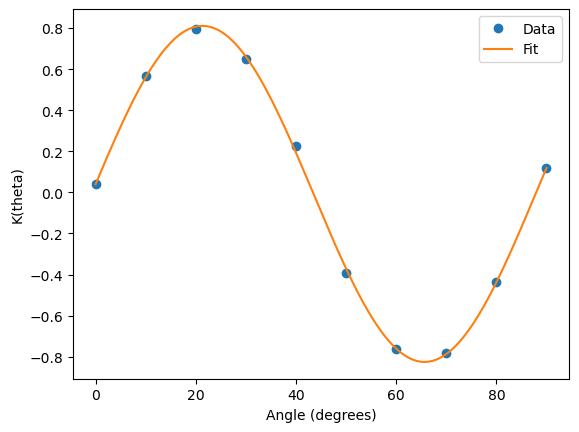
\includegraphics[width=\textwidth]{figures/fit_2.png}
        \caption{Fit for the second case.}
        \label{fig:fit_2}
    \end{subfigure}
    \caption{Comparison of fits for the first and second cases.}
    \label{fig:fit_comparison}
\end{figure}



Discussion on the necessity of two correlation functions for entanglement detection.

Calculation of visibility using the provided fit function.


\subsection{Violation of Bell’s Inequality}
Experimental settings for Alice and Bob’s angles.

Calculation of correlation functions and error propagation.

Interpretation of results demonstrating Bell inequality violation.

\subsection{Quantum State Tomography}
Measurement procedure for the four Bell states (\(|\phi^+\rangle\), \(|\phi^-\rangle\), \(|\psi^+\rangle\), \(|\psi^-\rangle\)).

Reconstruction of density matrices from experimental data.

Calculation of fidelity, purity, and eigenvalues.

Proof of entanglement using PPT criterion and entanglement witnesses.